\documentclass{sig-alternate}
\usepackage{amssymb,amsmath}
\usepackage{cleveref}
\usepackage{algorithm}
\usepackage{times}
\usepackage{color}
\usepackage{url}
\usepackage{subfigure}
\usepackage{xspace}
\usepackage[noend]{algorithmic}
\usepackage{enumerate}
\usepackage{multirow}
\usepackage{balance} 
\usepackage{epstopdf}

\newcommand{\squishlist}{
   \begin{list}{$\bullet$}
    {
      \setlength{\itemsep}{0pt}
      \setlength{\parsep}{3pt}
      \setlength{\topsep}{3pt}
      \setlength{\partopsep}{0pt}
      \setlength{\leftmargin}{1.5em}
      \setlength{\labelwidth}{1em}
      \setlength{\labelsep}{0.5em} } }

\newcommand{\squishend}{
    \end{list}  }


\newcommand{\model}{{S-STAT}\xspace} %stat is an abbreviation for statim which means immediately in latin
\newcommand{\w}{{\bf w}}
\newcommand{\z}{{\bf z}}
\newcommand{\loc}{{\bf l}}
\newcommand{\tim}{{\bf t}}

\newtheorem{definition}{Definition}

\begin{document}

\conferenceinfo{KDD`14}{August 22-27, 2014, New York City, New York USA}
%\CopyrightYear{2007} % Allows default copyright year (20XX) to be over-ridden - IF NEED BE.
%\crdata{0-12345-67-8/90/01}  % Allows default copyright data (0-89791-88-6/97/05) to be over-ridden - IF NEED BE.
% --- End of Author Metadata ---

\title{\model: Forecasting Rare Disease Outbreaks with Source Based Spatio-temporal Topic Models}

\numberofauthors{6}
%\author{
%% 1st. author
%\alignauthor
%Ben Trovato\titlenote{Dr.~Trovato insisted his name be first.}\\
%       \affaddr{Institute for Clarity in Documentation}\\
%       \affaddr{1932 Wallamaloo Lane}\\
%       \affaddr{Wallamaloo, New Zealand}\\
%       \email{trovato@corporation.com}
%% 2nd. author
%\alignauthor
%G.K.M. Tobin\titlenote{The secretary disavows
%any knowledge of this author's actions.}\\
%       \affaddr{Institute for Clarity in Documentation}\\
%       \affaddr{P.O. Box 1212}\\
%       \affaddr{Dublin, Ohio 43017-6221}\\
%       \email{webmaster@marysville-ohio.com}
%% 3rd. author
%\alignauthor Lars Th{\o}rv{\"a}ld\titlenote{This author is the
%one who did all the really hard work.}\\
%       \affaddr{The Th{\o}rv{\"a}ld Group}\\
%       \affaddr{1 Th{\o}rv{\"a}ld Circle}\\
%       \affaddr{Hekla, Iceland}\\
%       \email{larst@affiliation.org}
%\and  % use '\and' if you need 'another row' of author names
%% 4th. author
%\alignauthor Lawrence P. Leipuner\\
%       \affaddr{Brookhaven Laboratories}\\
%       \affaddr{Brookhaven National Lab}\\
%       \affaddr{P.O. Box 5000}\\
%       \email{lleipuner@researchlabs.org}
%% 5th. author
%\alignauthor Sean Fogarty\\
%       \affaddr{NASA Ames Research Center}\\
%       \affaddr{Moffett Field}\\
%       \affaddr{California 94035}\\
%       \email{fogartys@amesres.org}
%% 6th. author
%\alignauthor Charles Ptexalmer\\
%       \affaddr{Palmer Research Laboratories}\\
%       \affaddr{8600 Datapoint Drive}\\
%       \affaddr{San Antonio, Texas 78229}\\
%       \email{cpalmer@prl.com}
%}

\maketitle
\begin{abstract}
Rapidly increasing volumes of news feeds from diverse data sources, such as online newspapers, Twitter and online blogs are proving to be extremely valuable resources in helping anticipate, detect, and forecast outbreaks of rare diseases. Especially, aggregating and analyzing the shared information from all available data sources collectively enables the effective monitoring of disease emergence and progression.

In this paper, we introduce a spatio-temporal topic model over data sources that captures not only the low-dimensional structure of data, but also the spatial and temporal topic trends. The new model is capable of discovering the location and topic focus of each source, allowing us to use sources as experts with varying degrees of authoritativeness when predicting disease outbreaks. More precisely, we integrate the proposed topic model with one-class SVMs, so that modeling the underlying topic evolution and forecasting its prominence can be used as a surrogate for making near-term predictions of disease outbreaks. Finally, we employ a multiplicative weights algorithm to fuse the predictions from different sources for obtaining a final outbreak prediction while taking into account the accuracy of each individual source. We demonstrate the effectiveness of our proposed techniques using incidence data for Hantavirus in multiple countries of Latin America over a timespan of one year.
\end{abstract}

% A category with the (minimum) three required fields
\category{I.2.6}{Artificial Intelligence}{Learning}
%A category including the fourth, optional field follows...
\category{H.2.8}{Database Management}{Database Applications}[data mining] 

\terms{Algorithms, Experimentation}

\keywords{Graphical Models, Data Integration, Temporal Analysis, Topic Models}

\section{Introduction}
\label{sec:intro}
There has been a growing interest in developing statistical models for detecting infectious diseases as they arise, in a sufficiently timely fashion to enable effective control measures to be taken. Most of the early approaches targeted specific diseases and relied on highly specialized data, including medical records or environmental time series~\cite{wong:02,wong:03}.  Recently, however, there has been a growing interest in monitoring disease outbreaks using publicly available data on the Web, including news articles~\cite{brownstein:2008,linge:09}, blogs~\cite{corley:10}, search engine logs~\cite{ginsberg:09} and micro-blogging services, such as Twitter~\cite{culotta:2010}. Due to their volume, ease of availability, and ``citizen participation", such ``open source indicators" have been shown to be quite effective at monitoring disease emergence and progression.

Most of the proposed techniques rely on identifying specific keywords related to a set of predefined diseases and try to detect anomalous patterns over time with respect to the mention frequency of these keywords. While effective at detecting outbreaks of common diseases, such as influenza, the above techniques have significant limitations at predicting outbreaks of {\em rare}, yet deadly, diseases, such as Hantavirus. Since rare disease incidences are scarce, related keywords are sparsely distributed over time. Thus, it difficult for keyword based techniques to identify temporal patterns, and hence, detect the emergence of an outbreak in a timely manner. To address this limitation, researchers have employed models that identify temporal trends over {\em groups of words}, such as temporal topic models~\cite{paul:11} or frequent word-set mining~\cite{parker:13}. Both approaches rely on detecting co-occurence patterns of sets of words over time to discover the emergence and track the evolution of diseases. 

All of the aforementioned approaches are mainly used to detect generic disease trends and do not focus on location specific trends. However, rare disease topics may follow significantly different patterns when considering different locations. For example, Hantavirus outbreaks are more prominent in the Americas as opposed to Europe, and more notably, the rate of outbreaks across countries in the Americas varies significantly~\cite{jonsson:10}. Thus, not modeling the spatial correlations among disease outbreaks can confound outbreak patterns and result in unclear and sub-optimal location specific outbreak predictions. 

Finally, when analyzing publicly available data from multiple sources, it is of high-importance to consider the source lineage of information and take the quality (i.e., accuracy or authoritativeness) of each source into account when predicting disease outbreaks. For example, when monitoring and forecasting Hantavirus incidences in Chile, it is safer to consider analyzing data provided by localized sources, such as local news papers, than considering all Hantavirus-related news reported by source across the world. Nonetheless, all previous approaches assume all sources (e.g., blogs or Twitter users) have the same accuracy and consider the available data to its entirety when forecasting an outbreak. 

In this paper, we focus on the problem of providing location-specific disease outbreak predictions by analyzing a large corpus of publicly available health related news articles published by diverse data sources. More precisely, we model data sources as {\em evolving documents} over time, and introduce the {\em Source based Spatio-TemporAl Topic} model (\model), a topic  model that explicitly models time and location jointly with word co-occurence patterns. \model also models the correlations between locations and sources, enabling us to assess the authoritativeness and accuracy of each source for a specific location. The latter allows us to consider each source as an expert and fuse their individual predictions to obtain increased accuracy. 

At a high-level the model's generative process is as follows: Each data source is associated with a multinomial distribution over all available locations. A per-location multinomial distribution over topics is sampled from a Dirichlet prior, then for each entry provided by a data source a location is sampled by the source-specific location distribution, and a topic is sampled by the topic multinomial distribution corresponding to the assigned location; next two different per-topic multinomials generate the word and time point associated with each entry. This generative process naturally captures (a) the fact that most data sources, such as news papers, provide coverage only for a specific set of locations that is fixed over time, and (b) the fact that topics exhibit different prominence levels at different locations.

To predict a disease outbreak for a specific location at a future time point, we consider each source as an expert and integrate \model with one-class SVMs~\cite{schoelkopf:99} to detect any per source anomalous topic prominence that constitutes an early indicator of the onset of an outbreak. Finally, we employ a multiplicative weights algorithm~\cite{arora:2012} to learn the accuracy of each source and fuse the predictions corresponding to individual sources into a single final prediction using weighted majority voting.

The remainder of the paper is organized as follows: (a) we first provide an overview of the problem of rare disease forecasting by analyzing data from multiple sources (see \Cref{sec:problem}), (b) we then present an overview of the \model model (see \Cref{sec:model}), (c) followed by an experimental evaluation (see \Cref{sec:exp}) on the effectiveness of the proposed framework for forecasting Hantavirus outbreaks in Latin America by analyzing a corpus of public health-related news articles from January 2013 to January 2014, drawn from HealthMap \footnote{http://healthmap.org}~\cite{healthmap}, a prominent online source of news articles and tweets for disease outbreak monitoring and real-time surveillance of emerging public health threats.

\section{Problem Overview}
\label{sec:problem}

In this section, we formally define the problem of rare disease forecasting by analyzing data from multiple source. Consider we are given a collection of time-stamped event articles from a collection of data source $S$, referring to a set of locations $L$, containing words from a vocabulary $V$. We also consider a discrete time window $T$ containing a set of time points, so that the timestamp of each article can be associated with a single time point in $T$. For example, a time point $t \in T$ may correspond to a specific day or week over a time span of one year. For the remainder of the paper we will consider a time granularity is one week, defined as the 7-day period from Sunday to Saturday referred to as an {\em epidemiological week}, or {\em epi week} for short.

 It is convenient to convert the above input to a collection of tuples of the form {\em (source, location, word, time point; count)} where the count corresponds to the total number of articles mentioning a specific word and are associated with the source, location and time point in the tuple. For example, a tuple (``www.biobiochile.cl'', (``Los Lagos", ``Chile"), ``hanta", ``28''; 2) means that the count of news articles mentioning the word ``hanta" is two in the state of Los Lagos in Chile over the epi week 28.  

Given the input described above, we partition the data across the different sources in $S$ and view each source $s \in S$ as a collection of $N_s$ time-stamped event tuples, each of which is associated with a specific word, count, location and time point. Given this form of the input each source $s \in S$ can be viewed as a time-evolving document where multiple mentions of the same word for a specific location and time-point are aggregated into a unified entry in $N_s$. We also assume that each entry in $N_s$ is associated with a certain {\em latent topic}. Finally, let $\mathcal{X}$ denote the set of all event collections $N_s$ for all sources $s \in S$. For a particular set of event collections $\mathcal{X}$ our goal is to solve the following two problems:
\squishlist
\item {\bf Topic and Pattern Discovery.} Find the hidden topics that best summarize the events in $\mathcal{X}$, their temporal trends and hidden patterns, detect the topic prominence for each specific location, as well as, the location focus for each source.
\item {\bf Predicting Disease Outbreaks.} Forecast disease outbreaks for given future time points. 
\squishend
In the next two sections, we provide a detailed description of our proposed solutions to these two problems.

\section{Source Based Spatio-temporal \\ Topic Models}
\label{sec:model}
In this section we describe our method, \model, for dealing with the topic and pattern discovery problem. As mentioned before \model is a topic model that explicitly models time and location jointly with the word co-occurence patterns. Before introducing the \model model, we briefly review two topic models related to \model, i.e., the basic Latent Dirichlet Allocation (LDA) model~\cite{blei:2003} and the Author-Topic (AT) model~\cite{rosen:2004}. The graphical model representations of LDA and AT are shown in \Cref{fig:lda_model} and \Cref{fig:at_model} respectively.

LDA is a Bayesian network that generates a document using a mixture of topics. In its generative process, for each document $d$, a multinomial distribution $\theta_d$ over topics is randomly sampled from a Dirichlet with parameter $\alpha$, and then to generate each word, a topic $z_{di}$ is chosen from this topic distribution, and a word, $w_{di}$, is generated by randomly sampling from a topic-specific multinomial distribution $\phi_{z_{di}}$. The robustness of the model is greatly enhanced by integrating out uncertainty about the per-document topic distribution $\theta$ and the per-topic word distribution $\phi$. 

Rosen-Zvi et al., extended the basic LDA model by explicitly modeling author's interests as a mixture of topics. In its generative process for each document $d$, a set of authors $a_d$ is observed. To generate each word, an author $x$ is chosen uniformly from this set, then a topic $z_{di}$ is selected from a topic distribution $theta_{x}$ that is specific to the author, and then a word  $w{di}$ is generated from a topic-specific multinomial distribution $\phi_{z_{di}}$.

In \model, sources are viewed as dynamic documents and locations as authors similarly to the AT model. Moreover, topic discovery is influenced not only by word co-occurences, but also spatial and temporal information. Our notation is summarized in \Cref{tab:notation}, and the graphical model representation of \model is shown in \Cref{fig:stm_model}.  \model is a generative model of location, word, and time point in the timestamped event entries for all sources. Next, we describe the model's generative process used in Gibbs sampling for parameters estimation. The process is as follows: 

\begin{figure*}[ht]
\begin{center}
        \subfigure{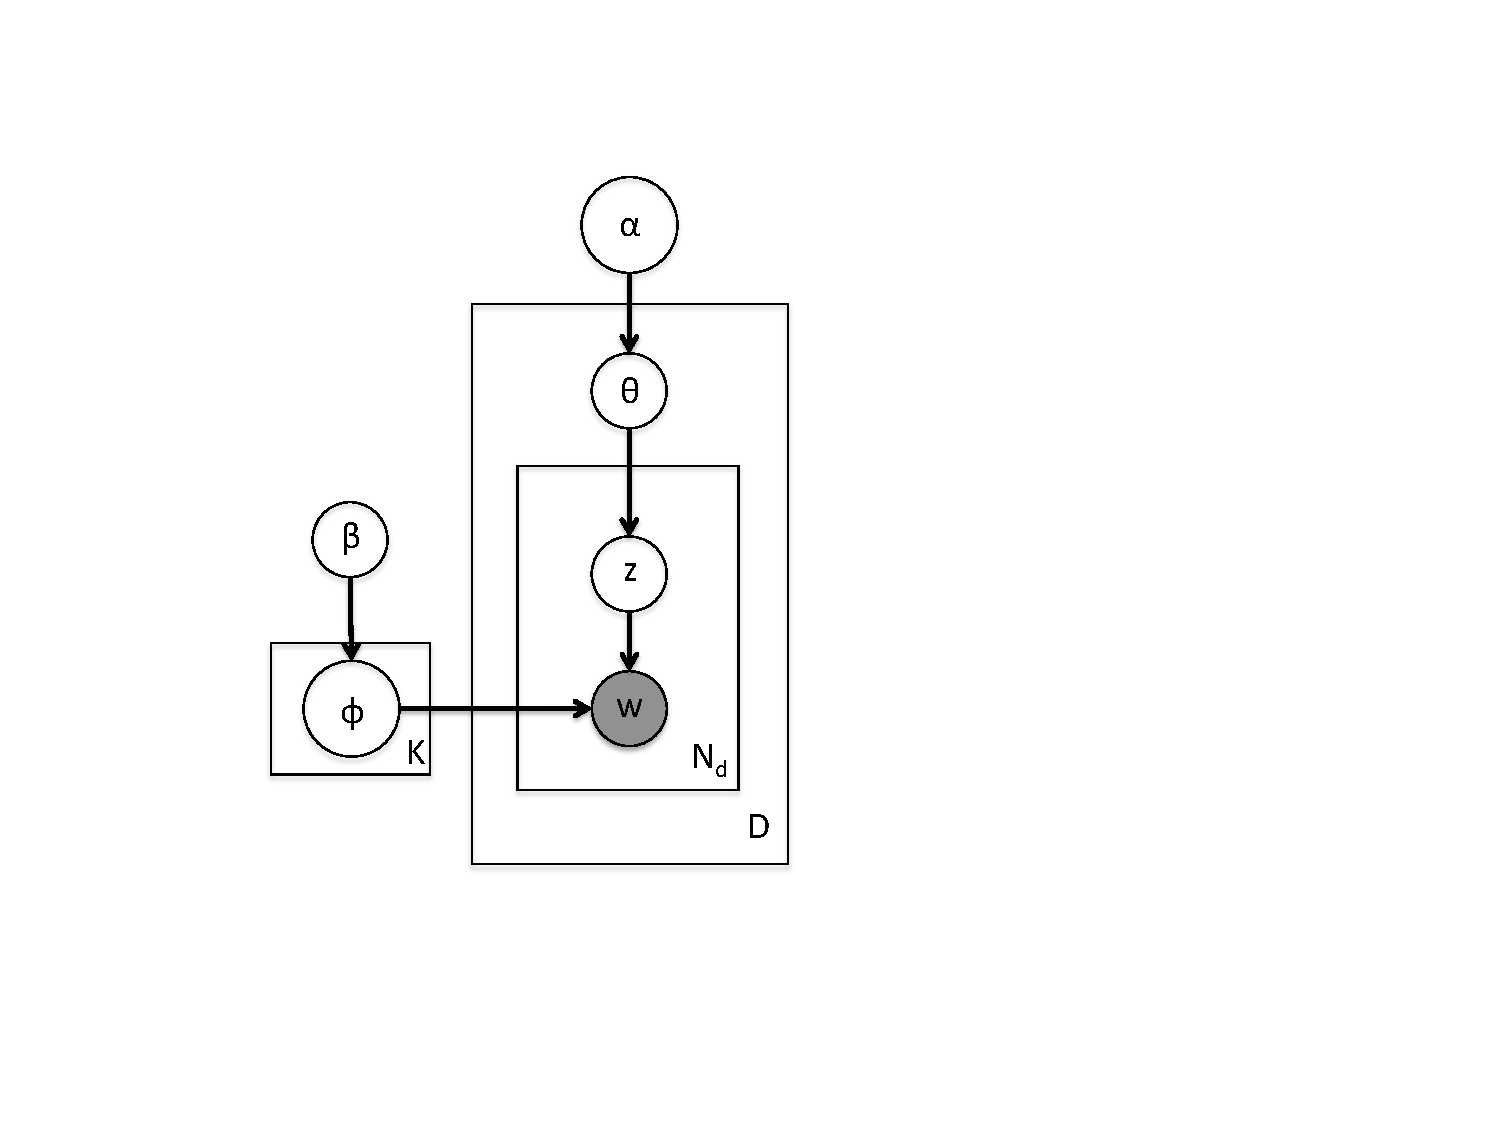
\includegraphics[trim = 40mm 35mm 80mm 25mm, clip, scale=0.4]{fig/lda_model.pdf} \label{fig:lda_model}}
        \subfigure{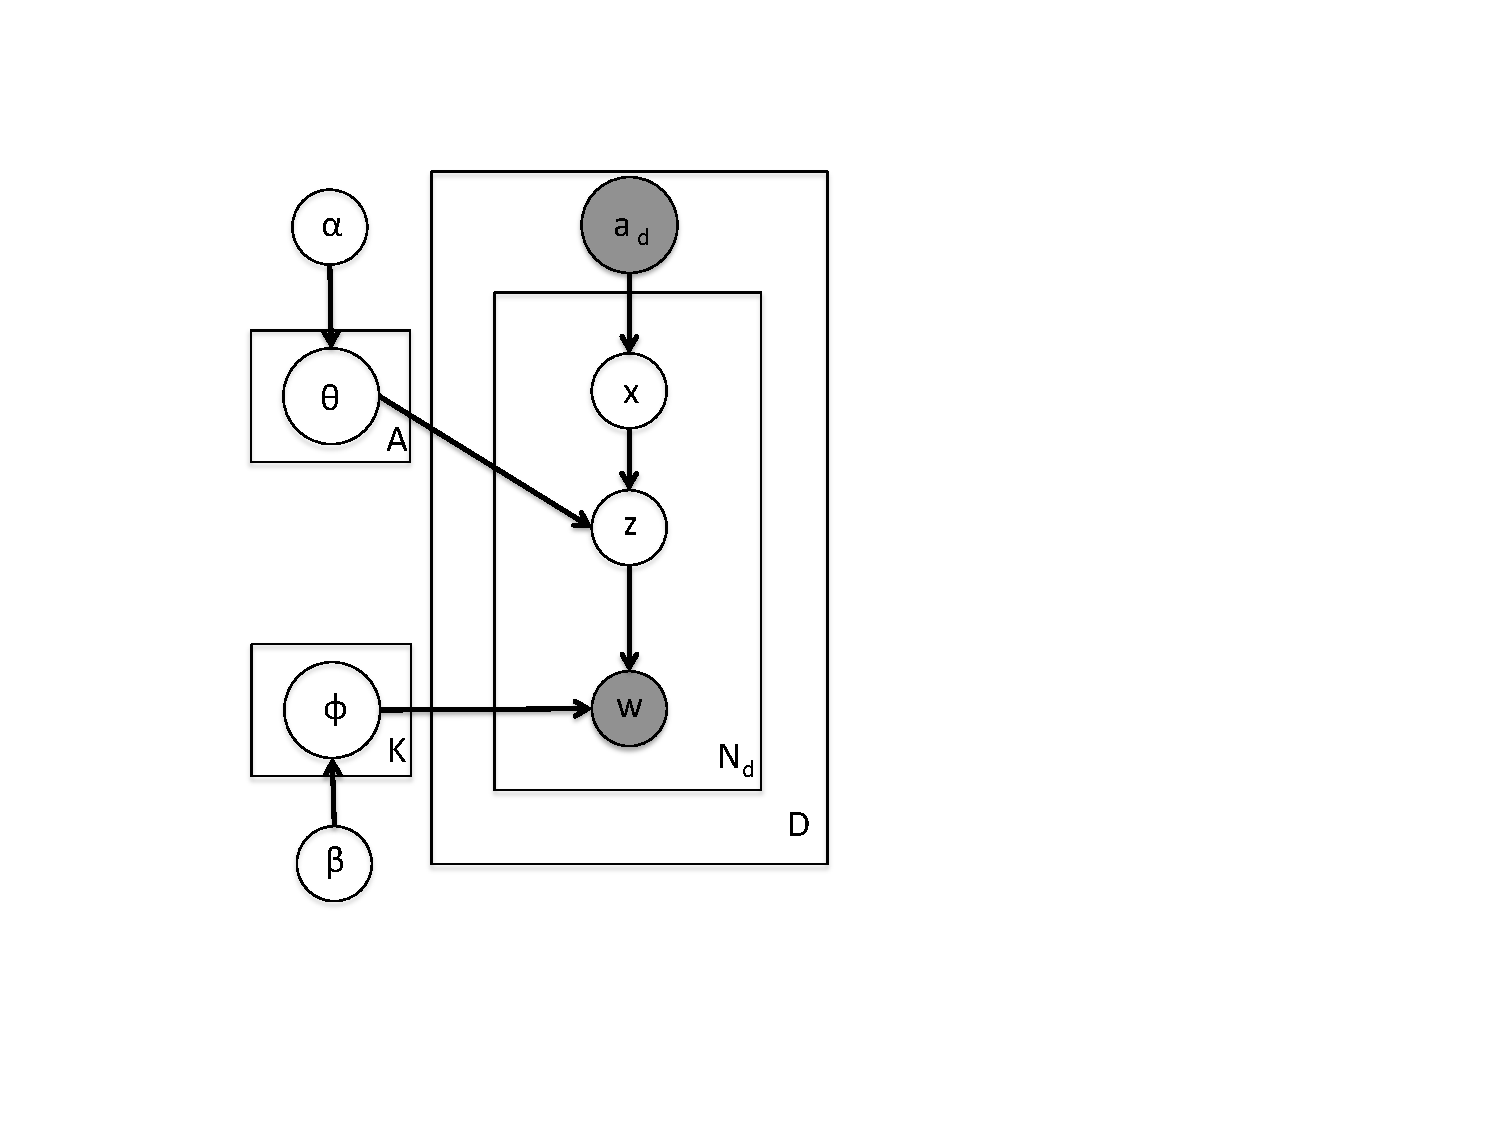
\includegraphics[trim = 40mm 35mm 70mm 25mm, clip, scale=0.4]{fig/at_model.pdf} \label{fig:at_model}}
        \subfigure{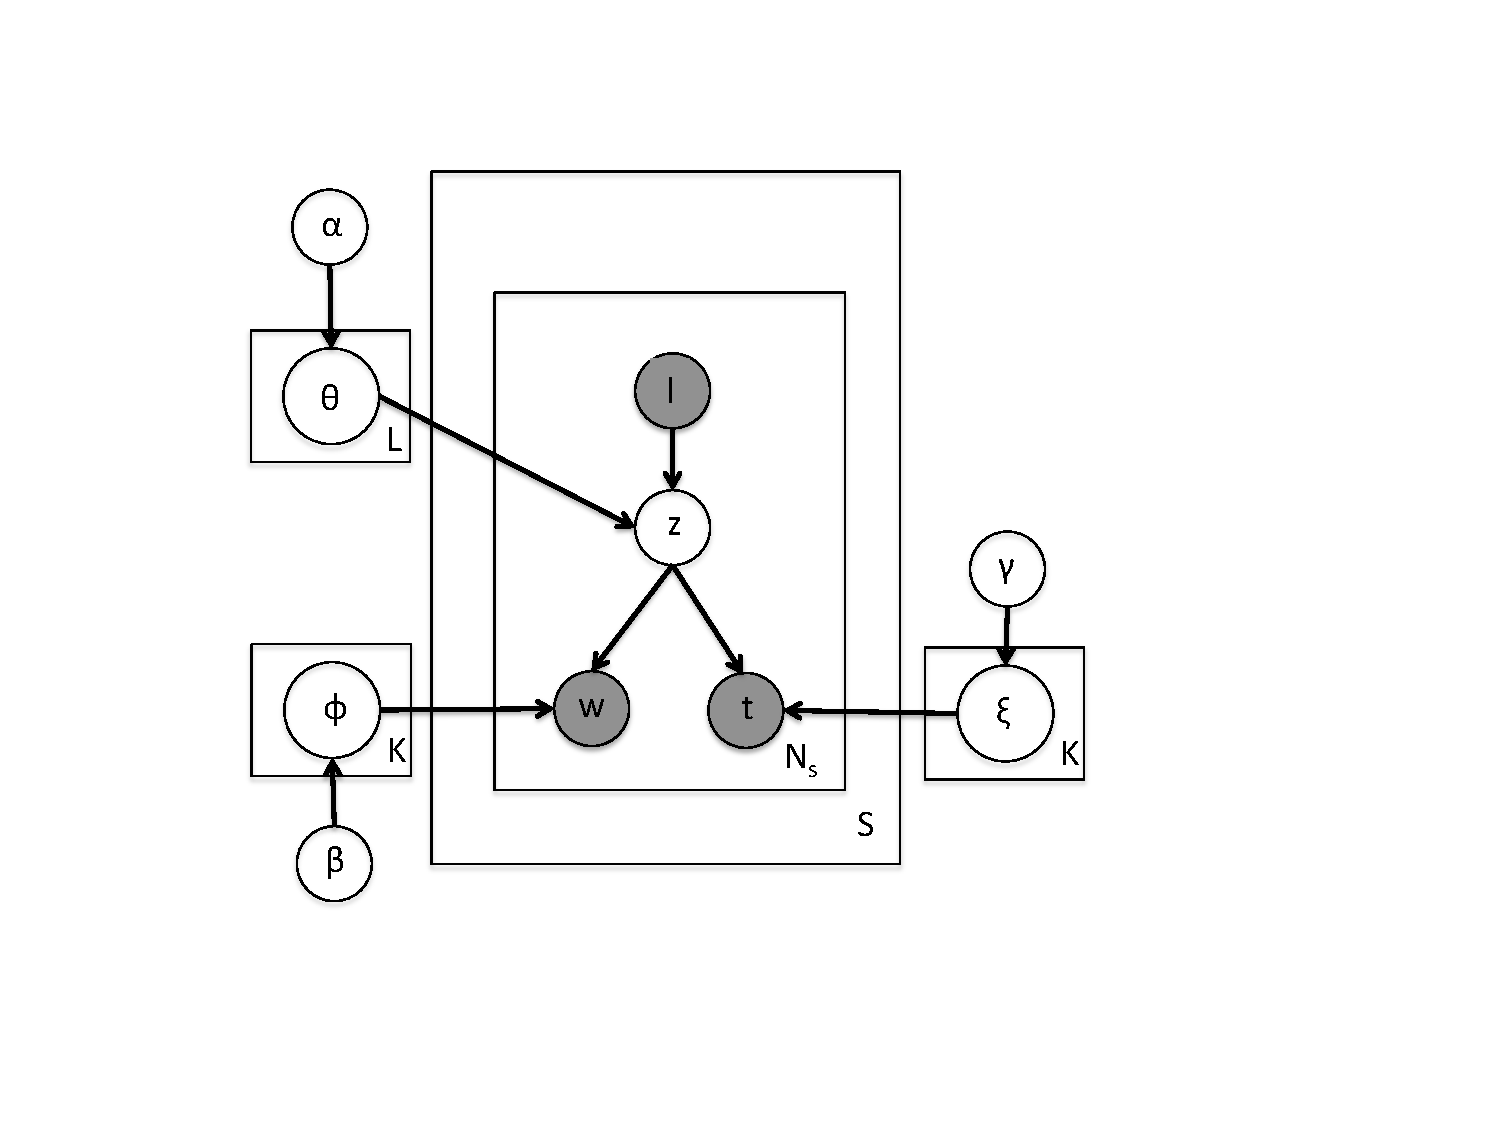
\includegraphics[trim = 30mm 35mm 70mm 25mm, clip, scale=0.4]{fig/stm_model.pdf} \label{fig:stm_model}}
\end{center}
\caption{Three topic models: (a) Latent Dirichlet Allocation Model. (b) Author-Topic Model. (c) S-STAT Model.}
\label{fig:models}
\end{figure*}


\begin{table}
\small \centering
\caption{Notation used in this paper.}
\begin{tabular}{c c}
\hline
{\bf Symbol} & {\bf Description}  \\
K & Number of topics  \\
S & Number of sources \\
V & Number of words \\
T & Number of discrete time-points \\
L & Number of locations \\
$N_s$ & Number of entries in each source $s$\\
$\psi_s$ & The multinomial distribution of locations specific to source $s$\\
$\theta_l$ & The multinomial distribution of topics specific to location $l$\\
$\phi_z$ & The multinomial distribution of words specific to topic $z$\\
$\xi_z$ & The multinomial distribution of time-points specific to topic $z$\\
$z_{si}$ & The topic associated with the $i$th entry from source $s$ \\
$l_{si}$ & The location associated with the $i$th entry from source $s$ \\
$w_{si}$ & The word associated with the $i$th entry from source $s$ \\
$t_{si}$ & The time-point associated with the $i$th entry from source $s$ \\
\hline
\end{tabular}
\label{tab:notation}
\end{table}

\ \\{\bf \model generative procees}
\begin{enumerate}
\item Draw $K$ multinomials $\phi_z$ from a Dirichlet prior $\beta$, one for each topic $z$;
\item Draw $K$ multinomials $\xi_z$ from a Dirichlet prior $\gamma$, one for each topic $z$;
\item Draw $L$ multinomials $\theta_l$ from a Dirichlet prior $\alpha$, one for each location $l$;
\item For each source  $s \in S$ and for each entry $i \in N_s$:
\begin{enumerate}
\item Draw a location $l$ from the multinomial $\psi_s$;
\item Draw a topic $z_{si}$ from the multinomial $\theta_l$;
\item Draw a word $w_{si}$ from multinomial $\phi_{z_{si}}$;
\item Draw a time-point $t_{si}$ from multinomial $\xi_{z_{si}}$.
\end{enumerate}
\end{enumerate}

We associate each source $s \in S$ with a multinomial distribution $\psi_s$ over all available locations mentioned in the available historical time-window. Moreover, for each location we consider a distribution $\theta_l$ over topics that is randomly sampled from a Dirichlet with parameter $\alpha$. To generate each entry $i \in N_s$ for source $s$, first, a location $l$ is chosen from the distribution $\psi_s$, and then a topic $z_{si}$ is chosen from the topic distribution $\theta_l$. Then, a word $w_{si}$ and time-point $t_{si}$ are generated by randomly sampling from the topic-specific multinomial distributions $\phi_{z_{si}}$ and $\xi_{z_{si}}$.  In our experiment we assume a fixed number of topics $K$.

As described in the above generative process, the posterior distribution of topics depends on the information from three modalities, i.e., the text, location and time. \model parametrization is:
\begin{align}
\theta_{l}|\alpha & \sim {\sf Dirichlet}(\alpha) \nonumber \\
\phi_{z}|\beta & \sim {\sf Dirichlet}(\beta) \nonumber \\ 
\xi_{z}|\gamma & \sim {\sf Dirichlet}(\gamma) \nonumber \\
l_{si}|\psi_s & \sim {\sf Multinomial}(\psi_s)  \nonumber \\
z_{si}|l,\theta_{l} & \sim {\sf Multinomial}(\theta_l) \nonumber \\
w_{si}|\phi_{z_{si}} & \sim {\sf Multinomial}(\phi_{z_{si}}) \nonumber \\
t_{si}|\xi_{z_{si}} & \sim {\sf Multinomial}(\xi_{z_{si}}) \nonumber
\end{align}

As inference cannot be done exactly in \model, we employ a Gibbs sampling algorithm to perform approximate inference. Using a Dirichlet conjugate prior for the multinomial distributions allows us to easily integrate out $\theta$, $\phi$ and $\xi$. The multinomial distribution over locations can be learned directly by the available data $N_s$ for each source. More precisely, given a source $s \in S$ we compute each parameter $p_{s,l}$ of the multinomial $\psi_s$  for each location $l \in L$ by taking its maximum likehood estimate, i.e., $p_{s,l} = {p}^{ML}_{s,l} = \frac{N_{l,s}}{N_{s}}$, where $N_{l,s}$ denotes the number of entries in $N_s$ associated with location $l$ and $N_s$ the total number of entries provided by source $s$.

In the Gibbs sampling procedure for estimating the parameters in \model, we need to calculate the conditional probability distribution $\Pr(z_{si}|{\bf w},{\bf t}, {\bf l}, {\bf z}_{-si}, \alpha, \beta, \gamma, {\bf \Psi})$ where ${\bf z}_{-si}$ represents the topic assignments for all entries in $s$ except the $i$-th entry. We begin with the joint probability of a data set and using the chain rule we obtain the conditional probability as:
\begin{align}
\label{eq:conditional}
&\Pr(z_{si}| \w,\tim,\loc,\z_{-si};\alpha,\beta,\gamma,\Psi) \nonumber \\
&= \frac{\Pr(z_{si}, w_{si}, t_{si}, l_{si}|\w_{-si},\tim_{-si},\loc_{-si},\z_{-si};\alpha,\beta,\gamma,\Psi)}{\Pr(w_{si}, t_{si}, l_{si}|\w_{-si},\tim_{-si},\loc_{-si},\z_{-si};\alpha,\beta,\gamma,\Psi)} \nonumber \\
& \propto \frac{n^{k,-(s,i)}_{w_{si}} + \beta_{w_{si}}}{\sum_{r = 1}^V n^{k,-(s,i)}_{r} + \beta_{r}} \cdot \frac{m^{k,-(s,i)}_{t_{si}} + \gamma_{t_{si}}}{\sum_{t = 1}^T m^{k,-(s,i)}_{t} + \gamma_{t}} \nonumber \\
& \cdot \frac{o^{k,-(s,i)}_{l_{si}} + \alpha_{l_{si}}}{\sum_{l = 1}^L o^{k,-(s,i)}_{l} + \alpha_{l}} \cdot \Pr(l_{si}|\psi_s)
\end{align}
where $n^{z}_{r}$ denotes the number of times word $r$ was associated with topic $z$ across all sources and entries, $m^{z}_{t}$ denotes the number of times time-point $t$ was associated with topic $z$ across all sources, $o^z_l$ denotes the number of times location $l$ was associated with topic $z$ across all sources and their entries, and $-si$ in the superscript indicates that the current example has been excluded by the count summations. A detailed derivation of Gibbs sampling for \model is provided in \Cref{sec:gibbs}. Once the sampler has converged, we can estimate the parameters of the multinomials $\theta$, $\phi$, and $\xi$ as follows:
\begin{align}
\label{eq:updates}
\theta_{l,z} = \frac{o^z_l + \alpha_l}{\sum_{z=1}^K o^z_l + \alpha_l} \nonumber \\
\phi_{z,v} = \frac{n^z_l + \alpha_l}{\sum_{v=1}^V n^z_v + \beta_v}  \\
\xi_{l,z} = \frac{m^z_t + \alpha_l}{\sum_{t=1}^T m^z_t + \gamma_t} \nonumber
\end{align}


The Gibbs sampling approximate inference for \model procedure is shown in Algorithm \ref{algo:gibbs}. For each entry in a set of event collection $\mathcal{X}$ we assign a hidden topic $z$ according to \Cref{eq:conditional}, and update the appropriate counts. After the sampling, we compute the distributions ${\boldsymbol \theta}$, ${\boldsymbol \xi}$ and ${\boldsymbol \phi}$ according to equation \Cref{eq:updates}. 

\begin{algorithm}[h]
\caption{\model Gibbs Sampling Approximate Inference}
\begin{algorithmic}[1]
\STATE {\bf Input:} $\mathcal{X}$: set of event entry collections; $N_{tier}$: number of iterations; ${\bf \Psi}$: source-location distributions;
\STATE {\bf Output:} ${\boldsymbol \theta}$: location-topic distributions; ${\boldsymbol \phi}$: topic-word distributions; ${\boldsymbol \xi}$: topic-timepoint distributions;
\STATE Initialize topic assignment randomly for all event entries in $\mathcal{X}$
\FORALL {$j$ to $N_{iter}$}
    \FORALL {$s \in S$}
    	\FORALL {$i \in N_s$}
		\STATE draw $z_{si}$ from $\Pr(z_{si}| \w,\tim,\loc,\z_{-si};\alpha,\beta,\gamma,\Psi)$
		\STATE update the counts $n^{z}_{r}$, $m^{z}_{t}$ and $o^z_l$
	\ENDFOR	
    \ENDFOR
\ENDFOR
\STATE Compute the posterior estimates ${\boldsymbol \theta}$, ${\boldsymbol \xi}$ and ${\boldsymbol \phi}$ as in \Cref{eq:updates}
\RETURN ${\boldsymbol \theta}$, ${\boldsymbol \xi}$, ${\boldsymbol \phi}$
\end{algorithmic}
\label{algo:gibbs}
\end{algorithm}


\section{Predicting Disease Outbreaks}
\label{sec:pred}
In the previous section we described how \model can be used to discover the topics and patterns in the available historical data. However, our final goal is to predict the emergence of disease outbreaks at future time points for each location $l \in L$. In this section, we describe how the posterior distributions learned by \model can be 
used to forecast outbreaks at a future time point $t$. We consider each source $s \in S$ to be an expert, providing predictions for a subset of locations $L_s \subseteq L$. We start with extracting individualized predictions for each source-location pair in $\mathcal{P} = \bigcup_{s \in S}s \times L_s$ by detecting if the source specific topic prominence for a certain location indicates an anomalous point, i.e., the incidence of a disease outbreak. Once all individualized predictions are extracted, we fuse all predictions corresponding to a location $l \in L$ using weighted majority voting. The weight of each source corresponds to its accuracy and authoritativeness for that particular location, and can be learned by historical data as we discuss below.

\subsection{Source-based Outbreak Predictions}
Predicting the incidence of an outbreak for a location $l$ at time $t$ given a source $s$, requires reasoning about the prominence of rare disease topics for $s$ at time $t$. Considering a source $s \in S$, we define the prominence of a topic $z \in K$ in $s$ at time $t$, as the {\em relevance} of topic $k$ to the content of $s$ at that time. Recall that for each topic $z \in K$, \model learns a distribution $\phi_z$ over all words in the vocabulary $V$. Similarly, given the set of words present in the articles provided by source $s$ for a location $l$ at time $t$, one can derive a source-location based distribution $P({\bf w};s,l,t)$ over all words in $V$ as described below.  Given $\phi_z$ and $P({\bf w};s,l,t)$ we define the relevance of a topic $z$ to source $s$ for location $l$ as the normalized distance between the distributions $\phi_z$ and $P({\bf w};s,l,t)$. Next, we discuss how the probability distribution $P({\bf w};s,l,t)$ can be estimated for future time points and we formally present a distance metric based on KL-divergence for defining relevance.

Given a source $s \in S$, a location $l \in L$ and a time point $t$ each parameters $p_{w,s,l,t}, \forall w \in V$ of the distribution $P({\bf w};s,l,t)$, can be estimated as $p_{w,s,l,t} = \frac{x_{w,s,l,t}}{\sum_{w \in V} x_{w,s,l,t}}$, i.e., the fraction of the number of articles $x_{w,s,l,t}$ by $s$ at time $t$ that correspond to location $l$ and mention the word $w$ over the total number of articles in $s$ at time $t$ for location $l$. Intuitively, when given a topic $z$ and a future time point $t$, the appearance count of a word in source $s$ for location $l$ at time $t$ is equal to the average occurrence rate of the word, regardless of the source, multiplied by the probability of that word being generated by topic $z$ multiplied by the probability that this topic is relevant to location $l$ and the probability of that topic being prominent at time $t$, multiplied by the probability of location $l$ appearing in $s$. Thus to compute the overall estimated appearance count of a word $w$ we need to sum over all topics. We have:

\begin{equation}
x_{w,s,l,t} = \bar{x}_{w}\cdot \sum_{z = 1}^K \phi_{z,w}\cdot \theta_{l,z} \cdot \xi_{z,t} \cdot \Pr(l|s) 
\label{eq:est_word}
\end{equation}
where $\bar{x}_{w}$ denotes the average rate of occurrences of word $w$ in $\mathcal{�}{X}$, and $\phi_{z,w}$, $\theta_{l,z}$, and $\Pr(l|s)$ can be retrieved by the distribution $\psi_s$ used in  \model. 

However, $\xi_{z,t}$, i.e., the probability of topic $z$ being prominent at time $t$, corresponds to a future time point and needs to be estimated. We use the values of distribution $\xi_{z}, \forall z \in K$ corresponding to past time points to forecast the values $\xi_{z,t} \mbox{with } z \in \{1, 2, \dots, K\}$. We use an autoregressive model over the values of topic $z$ for the $n$ previous time intervals, denoted by $\xi_{z,t-1},\xi_{z,t-2},\dots,\xi_{z,t-N}$.We have:
\begin{equation}
\xi_{z,t}=a_1 \cdot \xi_{z,t-1}+a_2\cdot \xi_{z,t-2}+\dots +a_n\cdot \xi_{z,t-n}
\end{equation}
where $a_1,a_2,.....,a_n$ are the regression coefficients.

To determine how relevant a topic is to the content of source $s$ for location $l$, we cast the problem as a document categorization topic and consider the normalized distance between distributions $\phi_z$ and $P({\bf w};s,l,t)$ to be equal to their symmetric KL distance~\cite{bigi:2003}.  More precisely, given a topic $z$ and the content of a source $s$ for location $l$ at time $t$, denoted by $s_{l,t}$ we have that the topic to source relevance is:

\begin{equation}
{\sf Relevance}(z, s_{l,t}) = 1 - \frac{KLD(\phi_z,s_{l,t})}{KLD(\phi_z,\emptyset)}
\end{equation}
where $KLD(\phi_z,s_{l,t})$ denotes the KL distance between distributions $\phi_z$ and $P({\bf w};s,l,t)$, and $KLD(\phi_z,\emptyset)$ denotes the KL distance between the distribution for topic $\phi_z$ and the empty document. For the empty document we define its word distribution as $P(w; \emptyset) = \epsilon, \forall w \in V$ where $\epsilon$ corresponds to a small positive constant. The symmetric KL distance between $\phi_z$ and $P({\bf w};s,l,t)$ is defined as:

\begin{equation}
KLD(\phi_z, s_{l,t}) = \sum_{w \in V} (P(w;z) - P(w;s,l,t))\cdot \log\frac{P(w;z)}{P(w;s,l,t)} \nonumber
\end{equation}
Due to space limitations we refer the reader to Bigi~\cite{bigi:2003} for details. 

Finally, to predict the incidence of a rare disease outbreak given a source $s$, a location $l$ and time $t$, we reason about the predicted relevance of rare disease topics to the sources content, detecting if the different topic relevance for each topic indicates an anomalous point, i.e., the incidence of a disease outbreak. To detect anomalous points we use one-class SVMs~\cite{schoelkopf:99} (OCSVM). A OCSVM maps input data $X$ into a high dimensional feature space $H$ via a kernel $\Phi: X \rightarrow H$ and finds the maximal margin hyperplane which best separates the training data from the origin. The classification rule corresponds to $f(x) = {\sf sign}(\mathbf{w}\Phi(x) - b)$, where $\mathbf{w}$ is a weight vector and $b$ is a bias term. We use this classification rule to detect if a new point $x$ is an anomalous point (i.e., $f(x) < 0$) or not. The sets of training examples for each of these OCSVMs is comprised by the predicted rare disease topic relevances for each source-location over the time points in the time window $T$.  

Recall that our goal is to detect the incidence of a particular disease outbreak for a specific location in $L$ given a source $s$. Operationally, we train a separate OCSVM for each source, location and disease triplet and forecast outbreaks on a weekly basis. To improve the robustness of each OCSVM, we excluding the time points that correspond to actual disease outbreaks from our training data. For this, we make use of a gold standard report (GSR) which gives ground truth determinations of whether a disease incidence (Hantavirus) happened in a given location at a time point included in $T$. The GSR is determined by analysts poring over multiple news sources and studying bulletins
issued by health reporting organizations such as ProMED~\cite{probmed}. 

This approach thus predicts  {\em if} a disease outbreak will happen based on the data provided by a source and {\em where} it will happen (since we are training and forecasting for each location). For the {\em when} since we are predicting for an epi week we adopt a standard relative date within the epi week to be the date at which the rare disease incidence will occur, and tune it using cross-validation. 



\subsection{Fusing Multiple Predictions}
\label{sec:integration}

Until now, we discussed how the events provided by each source can be used to derive an outbreak prediction when considering each individual source as an expert. However, our final goal is to detect the incidence of a particular disease for a specific location. Thus, we fuse the predictions of all sources into a single prediction for each location $l \in L$ at time $t$ using a {\em weighted majority voting algorithm} based on the multiplicative weights algorithm.

For time $t$ in the future, we focus on a location $l$ and view each source $s \in S$ as an expert providing a prediction $d_s \in [-1,1]$ for a disease emerging or not. We also assign a weight $w_s$ to each source. Given the predictions of all sources, we predict yes/no for an outbreak at location $l$ by taking the majority vote $\sum_{s \in S} w_s \cdot d_s$. 

Notice that for a certain location and time point not all sources may provide information for location that location. In fact it might be the case that through out the available historical time points a 

The weight $w_s$ of each source can be viewed as the {\em } of source's $s$ predictions for location $l$, denoted by $acc(s,l)$. More, precisely we define the accuracy of a source $s$ for a location $l$ as: 
\begin{equation}
acc(s,l) = coverage(s,l) \times precision(s,l)
\end{equation}
where $coverage(s,l)$ corresponds to the probability of location $l$ being mentioned in source $s$ and $precision(s,l)$ quantifies how accurate the predictions of source $s$ are for location $l$ given that $l$ was mentioned in $s$. 

Notice that the coverage of a source $s$ for all locations $l \in L$ corresponds to the probability distribution $\psi_s$ in the \model model, and can be learned directly by the input historical data. However, the precision of each source 

\section{Experimental Evaluation}
\label{sec:exp}

\ \\Basic results (quality, accuracy, recall, precision)

\ \\Source-location focus

\ \\Topics over time

\section{Related Work}
\label{sec:related_work}

\ \\Discuss basic LDA model

\ \\Discuss topics-over time, trimine, author-topic-model

\ \\Discuss anomaly detection


\section{Conclusions}
\label{sec:conclusion}

\bibliographystyle{abbrv}
\bibliography{src_tm.bib}

\appendix
\section{Gibbs Sampling for \model}
\label{sec:gibbs}
In this section we first provide a Gibbs sampling algorithm for learning the parameters of the \model model. Before we proceed with the actual algorithm we present the joint distribution corresponding to the \model model. We have the following:
{\scriptsize
\begin{align}
&\Pr(\w,\tim,\loc,\z,{\bf \phi},{\bf \theta},{\bf \xi};\alpha,\beta,\gamma,\Psi) =  \nonumber \\
&=\prod_{z = 1}^{K}\Pr(\phi_z;\beta)\Pr(\xi_z;\gamma) \prod_{l = 1}^{L}\Pr(\theta_l;\alpha) \nonumber \\
& \cdot \prod_{s = 1}^{S}\prod_{i = 1}^{N_s} \Pr(z_{si}|l_{si},\theta_l)\Pr(l_{si}|\psi_s)\Pr(w_{si}|\phi_{z_{si}})\Pr(t_{si}|\xi_{z_{si}}) \nonumber
\end{align}}
Next, we marginalize over all ${\bf \phi}$, ${\bf \xi}$ and ${\bf \theta}$. We have:
{\scriptsize
\begin{align}
&\Pr(\w,\tim,\loc,\z;\alpha,\beta,\gamma,\Psi) =  \int_{\phi}\int_{\theta}\int_{\xi} \Pr(\w,\tim,\loc,\z,{\bf \phi},{\bf \theta},{\bf \xi};\alpha,\beta,\gamma,\Psi) d\xi d\theta d\phi \nonumber \\
&=\int_{\phi} \prod_{z = 1}^{K}\Pr(\phi_z;\beta) \prod_{s = 1}^{S}\prod_{i = 1}^{N_s}\Pr(w_{si}|\phi_{z_{si}}) d\phi \nonumber \\
& \cdot \int_{\xi} \prod_{z = 1}^{K} \Pr(\xi_z;\gamma)\prod_{s = 1}^{S}\prod_{i = 1}^{N_s}\Pr(t_{si}|\xi_{z_{si}}) d\xi \nonumber \\
&\cdot \int_{\theta} \prod_{l = 1}^{L}\Pr(\theta_l;\alpha)\prod_{s = 1}^{S}\prod_{i = 1}^{N_s}\Pr(z_{si}|l_{si},\theta_{l_{si}})\Pr(l_{si}|\psi_s) d\theta \nonumber \\
&=\int_{\phi} \prod_{z = 1}^{K}\Pr(\phi_z;\beta) \prod_{s = 1}^{S}\prod_{i = 1}^{N_s}\Pr(w_{si}|\phi_{z_{si}}) d\phi \nonumber \\
&  \cdot \int_{\xi} \prod_{z = 1}^{K} \Pr(\xi_z;\gamma)\prod_{s = 1}^{S}\prod_{i = 1}^{N_s}\Pr(t_{si}|\xi_{z_{si}}) d\xi \nonumber \\
&\cdot \int_{\theta} \prod_{l = 1}^{L}\Pr(\theta_l;\alpha)\prod_{s = 1}^{S}\prod_{i = 1}^{N_s}\Pr(z_{si}|l_{si},\theta_{l_{si}}) d\theta \prod_{s = 1}^{S}\prod_{i = 1}^{N_s} \Pr(l_{si}|\psi_s)\nonumber
\end{align}
}
We focus on the different integrals in the expression presented above. We start with the integral over ${\bf \phi}$. 
{\scriptsize
\begin{align}
& \int_{\phi} \prod_{z = 1}^{K}\Pr(\phi_z;\beta) \prod_{s = 1}^{S}\prod_{i = 1}^{N_s}\Pr(w_{si}|\phi_{z_{si}}) d\phi \nonumber \\
& =  \prod_{z = 1}^{K} \int_{\phi_{z}} \Pr(\phi_z;\beta) \prod_{s = 1}^{S}\prod_{i = 1}^{N_s}\Pr(w_{si}|\phi_{z_{si}}) d\phi_{z} \nonumber \\
&= \prod_{z = 1}^{K} \int_{\phi_z} \frac{\Gamma(\sum_{r = 1}^V \beta_r)}{\prod_{r = 1}^V \Gamma(\beta_r)}\prod_{r = 1}^V \phi_{zr}^{\beta_r -1} \prod_{r = 1}^V \phi_{zr}^{n^{z}_{(\cdot),r}} d\phi_z \nonumber \\
&= \prod_{z = 1}^{K} \int_{\phi_z} \frac{\Gamma(\sum_{r = 1}^V \beta_r)}{\prod_{r = 1}^V \Gamma(\beta_r)}\prod_{r = 1}^V \phi_{zr}^{\beta_r  + n^{z}_{r} -1} d\phi_z \nonumber \\
& = \prod_{z = 1}^K \frac{\Gamma(\sum_{r = 1}^V \beta_r)}{\prod_{r = 1}^V \Gamma(\beta_r)} \frac{\prod_{r = 1}^V \Gamma(n^{z}_{r} + \beta_r)}{\Gamma(\sum_{r =1}^V n^{z}_{r} + \beta_r)} \nonumber
\end{align}}
where $n^{z}_{r}$ denotes the number of times word $r$ was associated with topic $z$ across all sources and entries. Similarly we have for the $\xi$ part:
{\scriptsize
\begin{align}
&\int_{\xi} \prod_{z = 1}^{K} \Pr(\xi_z;\gamma)\prod_{s = 1}^{S}\prod_{i = 1}^{N_s}\Pr(t_{si}|\xi_{z_{si}}) d\xi \nonumber \\
&= \prod_{z = 1}^K \int_{\xi_z} \Pr(\xi_z;\gamma)\prod_{s = 1}^{S}\prod_{i = 1}^{N_s}\Pr(t_{si}|\xi_{z_{si}}) d\xi \nonumber \\
& = \prod_{z = 1}^K \frac{\Gamma(\sum_{t = 1}^T \gamma_t)}{\prod_{t = 1}^T \Gamma(\gamma_t)} \frac{\prod_{t = 1}^T \Gamma(m^{z}_{t} + \gamma_t)}{\Gamma(\sum_{t =1}^T m^{z}_{t} + \gamma_t)} \nonumber
\end{align}}
where $m^{z}_{t}$ denotes the number of times time-point $t$ was associated with topic $z$ across all sources. Finally, we focus on the $\theta$ integral. We follow a similar analysis and have the following:
{\scriptsize
\begin{align}
&\int_{\theta} \prod_{l = 1}^{L}\Pr(\theta_l;\alpha)\prod_{s = 1}^{S}\prod_{i = 1}^{N_s}\Pr(z_{si}|l_{si},\theta_{l_{si}}) d\theta \nonumber \\
&= \prod_{l = 1}^L \int_{\theta_l} \Pr(\theta_l;\alpha)\prod_{s = 1}^{S}\prod_{i = 1}^{N_s}\Pr(z_{si}|l_{si},\theta_{l_{si}}) d\theta_l \nonumber \\
& = \prod_{l =1}^L\int_{\theta_l} \frac{\Gamma(\sum_{z = 1}^K \alpha_z)}{\prod_{z = 1}^K \Gamma(\alpha_z)}\prod_{z = 1}^K \theta_{lz}^{\alpha_z -1}\prod_{z=1}^K\theta_{lz}^{o^z_{l}}d\theta_l \nonumber \\
&= \prod_{l =1}^L\int_{\theta_l} \frac{\Gamma(\sum_{z = 1}^K \alpha_z)}{\prod_{z = 1}^K \Gamma(\alpha_z)}\prod_{z = 1}^K \theta_{lz}^{\alpha_z  + o^z_{l}-1}d\theta_l \nonumber \\
& = \prod_{l =1}^L\frac{\Gamma(\sum_{z = 1}^K \alpha_z)}{\prod_{z = 1}^K \Gamma(\alpha_z)}\frac{\prod_{z=1}^K\Gamma(o^z_l + \alpha_z)}{\Gamma(\sum_{z = 1}^K o^z_l + \alpha_z)}\nonumber
\end{align}}
where $o^z_l$ denotes the number of times location $l$ was associated with topic $z$ across all sources and their entries. 
Eventually we have that the joint distribution is given by:
{\scriptsize
\begin{align}
&\Pr(\w,\tim,\loc,\z;\alpha,\beta,\gamma,\Psi) = \prod_{z = 1}^K \frac{\Gamma(\sum_{r = 1}^V \beta_r)}{\prod_{r = 1}^V \Gamma(\beta_r)} \frac{\prod_{r = 1}^V \Gamma(n^{z}_{r} + \beta_r)}{\Gamma(\sum_{r =1}^V n^{z}_{r} + \beta_r)} \nonumber \\
&\cdot \prod_{z = 1}^K \frac{\Gamma(\sum_{t = 1}^T \gamma_t)}{\prod_{t = 1}^T \Gamma(\gamma_t)} \frac{\prod_{t = 1}^T \Gamma(m^{z}_{t} + \gamma_t)}{\Gamma(\sum_{t =1}^T m^{z}_{t} + \gamma_t)} \nonumber \\
& \cdot \prod_{l =1}^L\frac{\Gamma(\sum_{z = 1}^K \alpha_z)}{\prod_{z = 1}^K \Gamma(\alpha_z)}\frac{\prod_{z=1}^K\Gamma(o^z_l + \alpha_z)}{\Gamma(\sum_{z = 1}^K o^z_l + \alpha_z)} \cdot \prod_{s = 1}^{S}\prod_{i = 1}^{N_s} \Pr(l_{si}|\psi_s) \nonumber
\end{align}}
The goal of Gibbs sampling is to approximate the conditional distribution $\Pr(\z | \w, \tim,\loc;\alpha,\beta,\gamma,\Psi)$. Using the chain rule we have the following for the conditional probability:
{\scriptsize
\begin{align}
&\Pr(z_{si}| \w,\tim,\loc,\z_{-si};\alpha,\beta,\gamma,\Psi) \nonumber \\
&= \frac{\Pr(z_{si}, w_{si}, t_{si}, l_{si}|\w_{-si},\tim_{-si},\loc_{-si},\z_{-si};\alpha,\beta,\gamma,\Psi)}{\Pr(w_{si}, t_{si}, l_{si}|\w_{-si},\tim_{-si},\loc_{-si},\z_{-si};\alpha,\beta,\gamma,\Psi)} \nonumber \\
& \propto \frac{n^{k,-(s,i)}_{w_{si}} + \beta_{w_{si}}}{\sum_{r = 1}^V n^{k,-(s,i)}_{r} + \beta_{r}} \cdot \frac{m^{k,-(s,i)}_{t_{si}} + \gamma_{t_{si}}}{\sum_{t = 1}^T m^{k,-(s,i)}_{t} + \gamma_{t}} \nonumber \\
& \cdot \frac{o^{k,-(s,i)}_{l_{si}} + \alpha_{l_{si}}}{\sum_{l = 1}^L o^{k,-(s,i)}_{l} + \alpha_{l}} \cdot \Pr(l_{si}|\psi_s) \nonumber
\end{align}}
where $-si$ in the superscript indicates that the current example has been excluded by the count summations. 
\end{document}
